% ****************************************************************************************************
\chapter[Interdependencies within Platform as a Service Business Models]{Interdependencies within Platform as a Service Business Models}\label{ch:cld}
% ****************************************************************************************************

\begin{flushright}{\slshape    
	We shape our buildings; thereafter, our buildings shape us.} \\ \medskip
	--- Winston Churchill
\end{flushright}

\noindent In this chapter the essential interdependencies, i.e. high-leverage interventions and policies, between the previously described classification criteria and characteristics are described and illustrated using the concept of system dynamics, more specifically by means of a \acf{CLD}. Thus the second sub-research question is answered. 

System dynamics is an approach to study complexity and was originally developed at the \ac{MIT} by Jay W. \citet{Forrester1961}. John D. \citeauthor{Sterman2000} applied system dynamics to business and organizational problems. A comprehensive \citep{Sterman2000} as well as brief \citep{Sterman2001} introductory guide are provided. In this thesis, the notation and guidelines provided by \citeauthor{Sterman2000} are used (cf. op. cit.). The ultimate purpose of a \ac{CLD} is the simplification of the reality depicted by means of defining suitable model boundaries. \acp{CLD} \textit{"can never be comprehensive (and you shouldn't try: modeling is the art of simplification). They are also never final, but always provisional"} \citep[p. 166]{Sterman2000}. An important aspect of causal relationships within \acp{CLD} which should always be borne in mind, is that the causal relationships are modeled ceteris paribus, which literally translates to 'with other things the same' or 'all other things being equal or held constant'. Here, \textit{"a positive link means that if the cause increases, the effect increases above what it would otherwise have been, and if the cause decreases, the effect decreases below what it would otherwise have been. \ldots\xspace A negative link means that if the cause increases, the effect decreases below what it would otherwise have been, and if the cause decreases, the effect increases above what it would otherwise have been"} \citep[p. 139]{Sterman2000}.

At the beginning of this chapter the causal relationships for the generic customer segment in the \ac{PaaS} domain are discussed. Then, interdependencies between the five given customer segments are pointed out. At the end of this chapter the overall \ac{CLD} is presented and explained.

\section{Generic Platform as a Service Customer Segment}\label{ch:cld:cs}

Based on the outcome of the first sub-research question, as well as using the information and insights gained from the 23 explorative case studies, the relationships in the domain of the \ac{PaaS} customer segment were identified as discussed below. As mentioned earlier, this process is by nature iterative and thereby also accords with the \ac{DSR} design cycle introduced by \citet{Hevner2004} and \citet{Hevner2007} and the \ac{DSR} methodology process model introduced by \citet{Peffers2007}. Also, the evaluation with the help of experts and a focus group was conducted iteratively, and the results discussed hereafter represent the final version. Any remarkable changes of the model that occurred during the origination process are mentioned where appropriate.

\begin{figure}[tb]
	\centering
	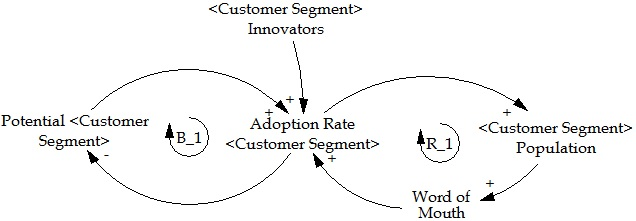
\includegraphics[width=0.8\textwidth]{gfx/cld_adoptionRate}
	\caption[Causal Loop Diagram -- Adoption Cycle]{Causal Loop Diagram -- Adoption Cycle, adopted from \citet[p. 18]{Sterman2001}}
	\label{fig:cld_ac}
\end{figure}

The core of the first sub-model, i.e. of the generic \ac{PaaS} customer segment (cf. Figure \ref{fig:cld_cs}), is the actual adoption process (cf. Figure \ref{fig:cld_ac}). This process is adopted from \citet[p. 18]{Sterman2001} and consists of the two main variables potential <customer segment>\footnote{The wildcard \texttt{<customer segment>} represents the five customer segments identified  earlier.} and the <customer segment> population which both are influenced by the adoption rate <customer segment> and vice versa. Given an increase in the <customer segment> population, the value of the favorable word of mouth variable will increase above what it would otherwise have been, and vice versa: if the <customer segment> population decreases, the value of the word of mouth variable will decrease below what it would otherwise have been. In the same vein, an increase or decrease in the value of the word of mouth variable will increase or decrease the value of the adoption rate <customer segment>. To close this first cycle, the adoption rate <customer segment> affects the <customer segment> population similarly, an increase in the adoption rate <customer segment> will increase the <customer segment> population above what it would otherwise have been, and obviously vice versa as well. So far, the first self-reinforcing feedback loop (labeled R\_1\footnote{R\_1: Adoption Rate <Customer Segment> -- <Customer Segment> Population -- Word of Mouth -- Adoption Rate <Customer Segment>}) in this model has been described. \citet[p. 19]{Sterman2001} calls this cycle \textit{"contagion loop"}. 

In the absence of external influences, a self-reinforcing feedback loop will make all variables involved grow exponentially. Obviously, the <customer segment> population cannot grow exponentially forever, and thus at least one variable of the self-reinforcing feedback loop needs to be influenced exogenously. In this particular case, the adoption rate <customer segment> is regulated through the variable potential <customer segment>. An increase in the adoption rate <customer segment> will decrease the variable potential <customer segment> below what it would otherwise have been, hence the negative link polarity from the adoption rate <customer segment> to the potential <customer segment>. The variable potential <customer segment> itself influences the adoption rate <customer segment> in a contrary way: a decrease in the number of potential <customer segment> will decrease the number of adopters (adoption rate <customer segment>) below what it would otherwise have been. Due to the fact that this feedback loop contains one link with a negative polarity, it is a balancing feedback loop (labeled B\_1\footnote{B\_1: Adoption Rate <Customer Segment> -- Potential <Customer Segment> -- Adoption Rate <Customer Segment>}), \citet[p. 18]{Sterman2001} named this loop \textit{"market saturation"}. This balancing feedback loop prevents the variable <customer segment> population to grow exponentially and adjusts the adoption rate <customer segment> correspondingly.

\begin{figure}[tb]
	\centering
	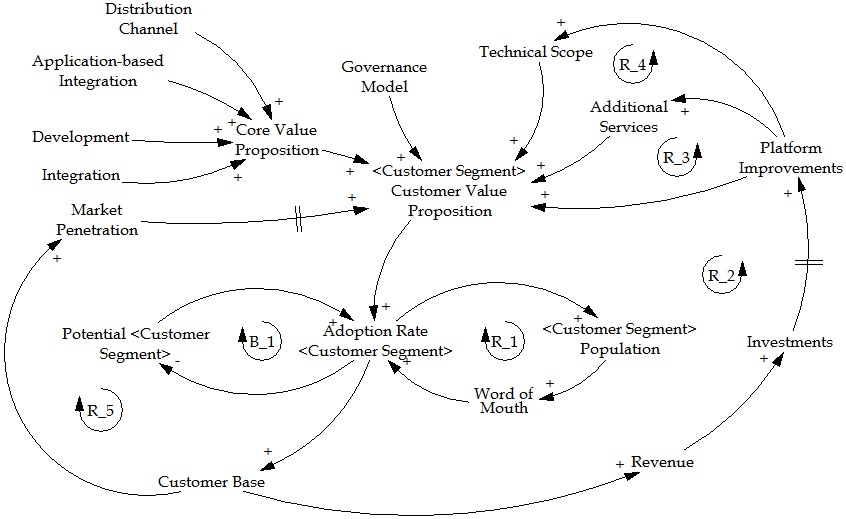
\includegraphics[width=\textwidth]{gfx/cld_customerSegment}
	\caption{Causal Loop Diagram -- Generic PaaS Customer Segment}
	\label{fig:cld_cs}
\end{figure}

In addition to the two above mentioned links to the adoption rate <customer segment>, the main link in the \ac{PaaS} domain is the influence of the <customer segment> customer value proposition (cf. Figure \ref{fig:cld_cs}). As discussed earlier, the business model conceptualization proposed by \citet{Johnson2008} emphasizes the need for a specific \ac{CVP} for each customer segment, so as to take the different customer needs into account explicitly. Thus, all five customer segments receive their own, unique \ac{CVP}. Naturally, the relationship between the <customer segment> customer value proposition and the adoption rate <customer segment> is a link with a positive polarity -- an increase in the <customer segment> customer value proposition will increase the adoption rate <customer segment> above what it would otherwise have been. During the evolution of the qualitative model, this aspect of the \ac{CVP} was discussed quite controversially. It was challenged whether it is necessary to have five \acp{CVP} in the model, one for each customer segment. Ultimately, however, an agreement was reached that considering five different \acp{CVP} is crucial to capturing the causal relationships in the \ac{PaaS} domain.

The <customer segment> customer value proposition itself is influenced by six factors: through the (1) core value proposition, (2) governance model, (3) technical scope, (4) additional services, (5) market penetration, and (6) platform improvements. During the analysis of the 23 explorative case studies, especially with regard to the \ac{CVP}, as well as during the development of the classification scheme, a correlation between the core value proposition and the <customer segment> customer value proposition was discovered. It has been argued that for the purpose of classifying \ac{PaaS} providers, a provider is classified mainly by one characteristic of the core value proposition. However, in case of the qualitative model the core value proposition of a \ac{PaaS} provider is composed of all four identified characteristics of the core value proposition.

Moreover, the <customer segment> customer value proposition is influenced by two further classification criteria, viz. governance model and technical scope. Both criteria are mapped onto an ordinal scale, so that modeling the impact on the <customer segment> customer value proposition is straightforward. An increase in the value of the technical scope or governance model will increase the <customer segment> customer value proposition above what it would otherwise have been. The two variables governance model and core value proposition (and its four influence variables) will remain constant, due to the fact that these variables are themselves not influenced by any other variables.

Another point which was discussed during the 	evolution of this qualitative model was how to include the previously identified revenue streams into the model. Based on the lack of knowledge of user preferences concerning the revenue streams, these are excluded from the model because they cannot be modeled realistically. Further research is necessary to determine which revenue streams are preferred by the \ac{PaaS} stockholders. However, the analysis of the 23 explorative case studies revealed that nearly all \ac{PaaS} providers offer additional products and especially services, for instance training, certifications, and consultancy services. Hence, it can be inferred that these extras (henceforth referred to as additional services) influence the <customer segment> customer value proposition favorably. An increase in the value of the additional services variable will therefore increase the value of the <customer segment> customer value proposition above what it would otherwise have been.

However, the adoption rate <customer segment> itself influences the variable customer base positively. An increase in the adoption rate <customer segment> will increase the customer base above what it would otherwise have been. The impacts of the variable customer base are twofold. 

First, an increase in the variable customer base will increase the variable revenue above what it would otherwise have been. In return, an increase in the variable revenue will increase the value of the variable investments above what it would otherwise have been. Further, an increase in the variable investments will increase the variable platform improvements delayed above what it would otherwise have been. This assumption chain is in accord with \citet[p. 200]{Evans2003}, who concluded that \textit{"many successful multi-sided firms have tested and modified their platforms with minimal investment and then scaled up according to what works best"}. The variable platform improvements itself influences three variables already mentioned above: <customer segment> customer value proposition, additional services, and technical scope. Thus three further self-reinforcing feedback loops are identified (labeled R\_2\footnote{R\_2: Customer Base -- Revenue -- Investments --- Platform Improvements -- <Customer Segment> Customer Value Proposition -- Adoption Rate <Customer Segment> -- Customer Base}, R\_3\footnote{R\_3: Customer Base -- Revenue -- Investments --- Platform Improvements -- Additional Services -- <Customer Segment> Customer Value Proposition -- Adoption Rate <Customer Segment> -- Customer Base}, and R\_4\footnote{R\_4: Customer Base -- Revenue -- Investments --- Platform Improvements -- Technical Scope -- <Customer Segment> Customer Value Proposition -- Adoption Rate <Customer Segment> -- Customer Base}).

The second impact of the variable customer base concerns the variable market penetration. An increase in the variable customer base will increase the variable market penetration above what it would otherwise have been. In the 23 explorative case studies it was remarkable that a company's brand image and the company's reputation was an important element of its \ac{CVP}. It can be concluded that this issue will influence the <customer segment> customer value proposition, even though this impact will occur with a delay. Hence, an increase in the variable market penetration will increase the variable <customer segment> customer value proposition delayed above what it would otherwise have been. The above described causal relationships constitute the fifth self-reinforcing feedback loop (labeled R\_5\footnote{R\_5: Customer Base -- Market Penetration --- <Customer Segment> Customer Value Proposition -- Adoption Rate <Customer Segment> -- Customer Base}).

\section{Platform as a Service Customer Segment Interdependencies}\label{ch:cld:csi}

In this section the interdependencies between the customer segments identified in Chapter \ref{ch:sota} are discussed and depicted in Figure \ref{fig:cld_csi}. \citet[p. 33]{Cusumano2010} reasons, that \textit{"the critical distinguishing feature of an industry platform and ecosystem is the creation of 'network effects'. These are positive feedback loops that can grow at geometrically increasing rates as adoption of the platform and the complements rise. The network effects can be very powerful \ldots~"}. The self-reinforcing feedback loop R\_1 described in the previous section represents a direct network effect, also known as same-side network effect. Gaming platforms are a well-known example of this network effect -- the more gamers use a certain platform, the more valuable the platform becomes for other gamers. However, the direct network effects in the \ac{PaaS} domain are not considered to be the decisive factor. In contrast, indirect network effects are likely to be one of the main decisive factors. In general, an indirect network effect arises when there are cross-sided network effects in both directions (from A to B and vice versa). Once again gaming platforms are used as case in point: The platform value for gamers depends among other things on the number of games available for the platform. On the other hand, these games are provided by game developers whose perceived platform value depends on the number of gamers using the platform. Frequently, such indirect network effects are accompanied by the so-called chicken-and-egg launch problem. 

Platform customers are characterized as upper \acp{SME} or large enterprises using the platform mainly for internal purposes. The introduction of a platform for these customers will most likely be an extensive project which is often supported externally through \acp{SI}. Therefore, an increase in the platform customer population will increase the systems integrator population above what it would otherwise have been. For reasons of clearer illustration the above-described causal relationship as well as the corresponding depiction in Figure \ref{fig:cld_csi} has been simplified. Actually, an increase in the platform customer population will increase the systems integrator customer value proposition, which in turn will increase the adoption rate systems integrator, which finally will increase the systems integrator population. This pattern of simplification also applies to the \ac{PaaS} customer segment dependencies discussed below.

In the opposite direction, an increase in the systems integrator population will increase the platform customer population above what it would otherwise have been. This causal relationship is considered weak since only very few potential platform customers will adopt the platform based on the existence of a large systems integrator population. Therefore it is represented by broken arrows in the diagram. However, even though this relationship is weak, a correlation can be noticed. Taken together the sixth self-reinforcing feedback loop has been found (labeled R\_6\footnote{R\_6: Platform Customer Population -- Systems Integrator Population - - Platform Customer Population}). The platform customer population is further influenced by the variable platform modules\footnote{Platform modules are defined as \textit{"an add-on software subsystem that connects to the platform to add functionality to the platform"} \citep[p. 676]{Tiwana2010}, cf. Section \ref{ch:tf:paas:def}.} as discussed further below.

\begin{figure}[tb]
	\centering
	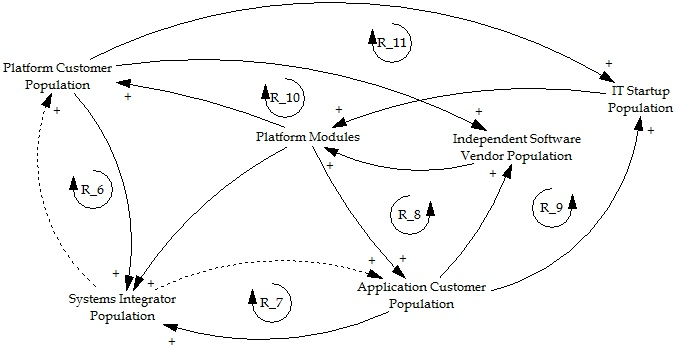
\includegraphics[width=\textwidth]{gfx/cld_customerSegmentInterdependencies}
	\caption{Causal Loop Diagram -- PaaS Customer Segment Interdependencies}
	\label{fig:cld_csi}
\end{figure}

A similar feedback loop can be identified between the systems integrator population and the application customer population. Also, the introduction of platform modules by application customers is occasionally supported by \acp{SI}. Therefore, an increase in the application customer population will increase the systems integrator population above what it would otherwise have been. As with the platform customers, the application customer population is influenced by the systems integrator population, although this causal connection is again relatively weak. The above mentioned correlation constitutes the seventh self-reinforcing feedback loop (labeled R\_7\footnote{R\_7: Application Customer Population -- Systems Integrator Population - - Application Customer Population}).

Moreover, the systems integrator population is also influenced by the variable platform modules. The number or the growth rate of the available platform modules commonly serves as a reliable indicator of a flourishing platform and corresponding ecosystem. Hence, an increase in the variable platform modules will increase the systems integrator population above what it would otherwise have been.

Platform modules, such as applications, services, components, and add-ons, are developed and provided by \acp{ISV} and \ac{IT} startups. Thus an increase in the \ac{IT} startup population or independent software vendor population will increase the variable platform modules above what it would otherwise have been. The variable platform modules itself influences the application customer population positively -- an increase in the variable platform modules will increase the application customer population above what it would otherwise have been. And finally, the application customer population influences both populations of providers of platform modules positively. An increase in the application customer population will increase the \ac{IT} startup population as well as the independent software vendor population above what it would otherwise have been. Thereby two further self-reinforcing feedback loops are disclosed (labeled R\_8\footnote{R\_8: Application Customer Population -- Independent Software Vendor Population -- Platform Modules -- Application Customer Population} and R\_9\footnote{R\_9: Application Customer Population -- \ac{IT} Startup Population -- Platform Modules -- Application Customer Population}).

As briefly mentioned above, the platform customer population is also influenced by the variable platform modules. Even though this customer group uses the platform mainly for internal projects, re-usable platform modules can rapidly accelerate the development of new solutions. Hence, an increase in the variable platform modules will increase the platform customer population above what it would otherwise have been. These platform modules are provided by \acp{ISV} and \ac{IT} startups and thus an increase in the platform customer population will increase the independent software vendor population as well as \ac{IT} startup population above what it would otherwise have been. Thus the last two self-reinforcing feedback loops within the second sub-model have been identified (labeled R\_10\footnote{R\_10: Platform Customer Population -- Independent Software Vendor Population -- Platform Modules -- Platform Customer Population} and R\_11\footnote{R\_11: Platform Customer Population -- \ac{IT} Startup Population -- Platform Modules -- Platform Customer Population}).

\section{The Big Picture}\label{ch:cld:bp}

Finally, the overall qualitative model, in other words the big picture (cf. Figure \ref{fig:cld_bp}), which is based on the two sub-models discussed above is presented. In this model, the generic \ac{PaaS} customer segment sub-model is included five times, corresponding to the five distinct customer segments. It should be noted that each customer segment now receives its own unique \ac{CVP}. This differentiation is in accord with \citet{Johnson2008}. It takes the varying \acp{CVP} into account and enables a proper modeling of this aspect. Moreover, the sub-model of the \ac{PaaS} customer segment interdependencies is also present in the overall model. However, in contrast to the sub-model of the \ac{PaaS} customer segment interdependencies, the relationships that were simplified in that model are represented in detail in the overall model. In Section \ref{ch:cld:csi} the above-mentioned simplification is discussed briefly.

All causal relationships presented in the overall model have already been introduced (cf. Section \ref{ch:cld:cs} and \ref{ch:cld:csi}) and therefore will not be explained again. As mentioned earlier, one important aspect of modeling consists in defining suitable model boundaries. A few design decisions made during the evolution of the qualitative model were mentioned already; now further challenges are discussed.

In this model, the aspect of revenue is only considered at a basic level\footnote{An increase in the customer base will increase the revenue above what it would otherwise have been and so forth, compare also the feedback loops R\_2, R\_3, and R\_4 within Figure \ref{fig:cld_cs}}, and the aspect of expenses, the importance of which is undeniable, is not considered at all. In order to do so, an unmanageable number of criteria would be necessary to model costs appropriately. For instance, expenses depend on the deployment model, location, size of the company, the number of developers, and other factors. The aspect of expenses with respect to the problem discussed here cannot be modeled adequately in the available time frame and is therefore excluded from the model.

Another aspect which is considered, if in simplified terms, represents the market penetration. In the model an increase in the customer base will increase the market penetration above what it would otherwise have been, and will thereby influence the corresponding \ac{CVP} positively, via the company's brand image and reputation. The value of the market penetration solely depends on the inherent model values, to be exact on the values of the potential <customer segment> and <customer segment> population. Actually, the value of the market penetration also depends crucially on the competition. The threat of new players and the rivalry among existing competitors \citep[pp. 80-82, 85-86]{Porter2008} are the most influential forces here. However, in order to model the \ac{PaaS} market in a proper way, various other model variables, such as the company's own market share, competition market share, threat of new competitors, and overall market penetration, as well as further assumptions are necessary. Attempting to add the whole \ac{PaaS} market to the model would be a complex task which would lie beyond the scope of this thesis. For this reason the \ac{PaaS} market in the overall model is represented in a simplified way through the variable market penetration. In the following Figure \ref{fig:cld_bp} the overall model, i.e. the big picture, is depicted:

\newpage

\ifthenelse{
	\isodd{\thepage}
}{%odd
	\begin{figure}[tb]
		\centering
		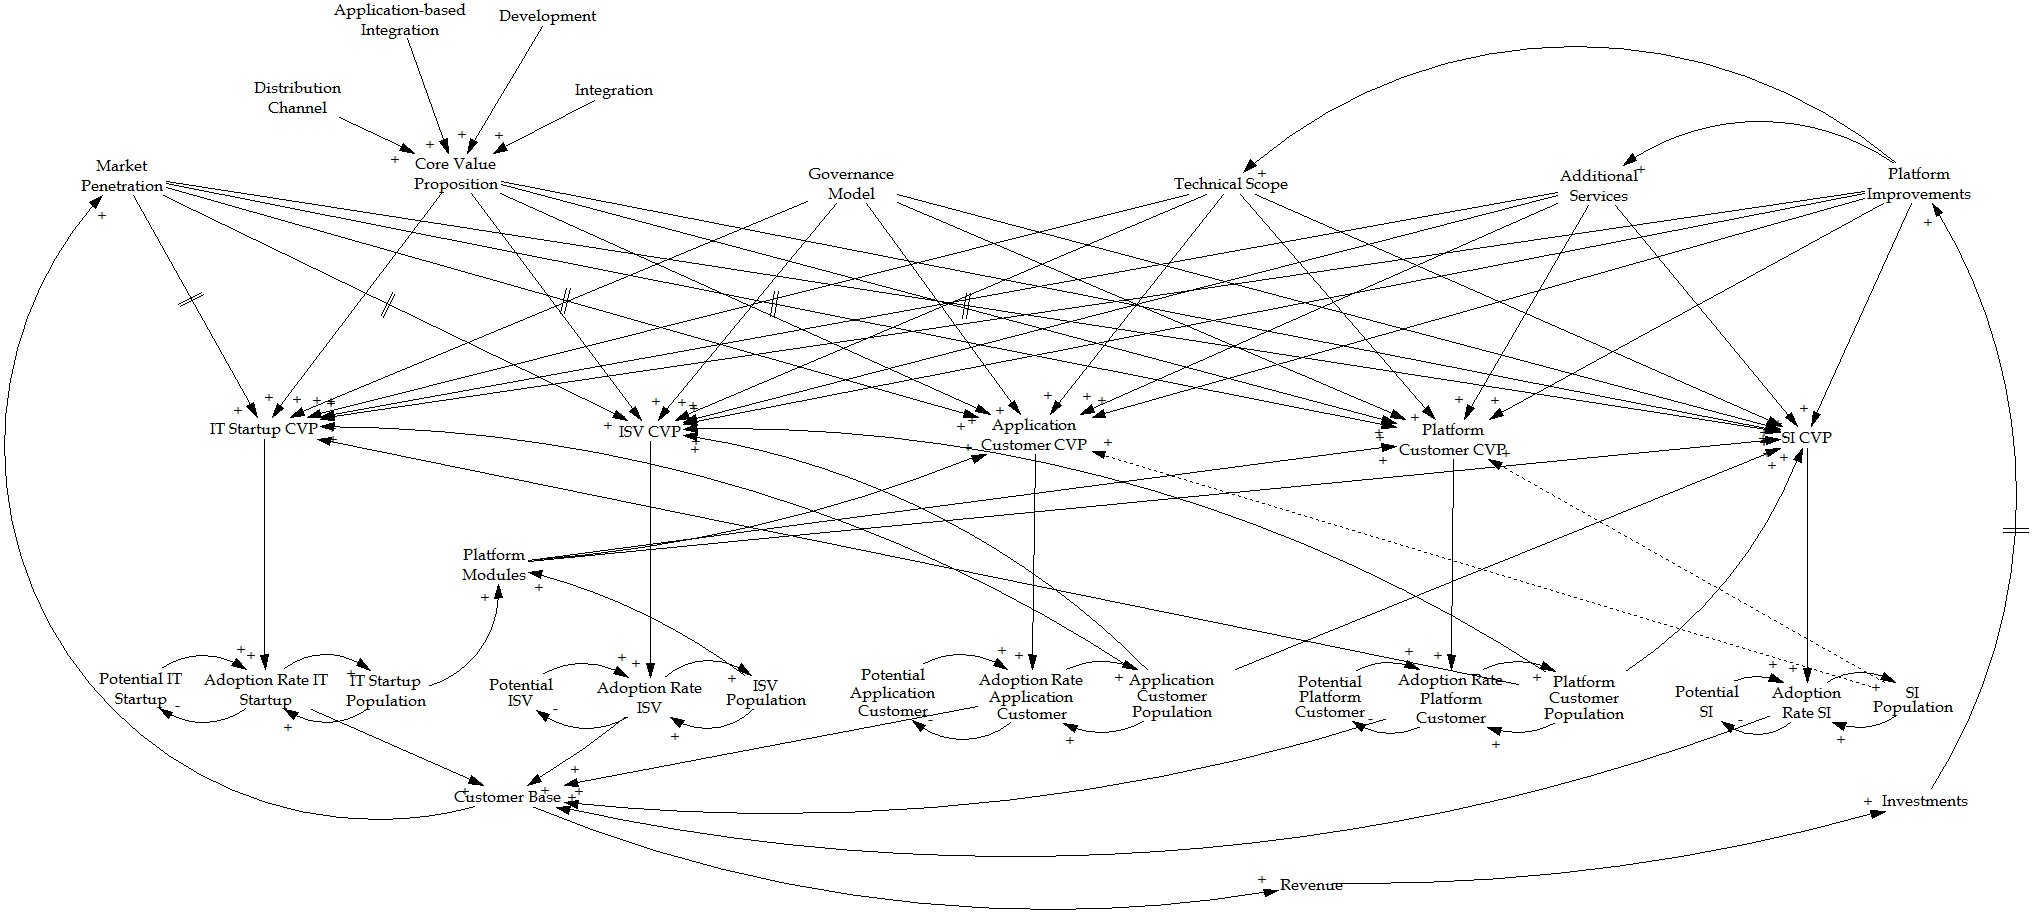
\includegraphics[width=0.96\textheight,angle=90]{gfx/cld_bigPicture}
		\caption{Causal Loop Diagram -- The Big Picture}
		\label{fig:cld_bp}
	\end{figure}
}{%even
	\begin{figure}[tb]
		\centering
		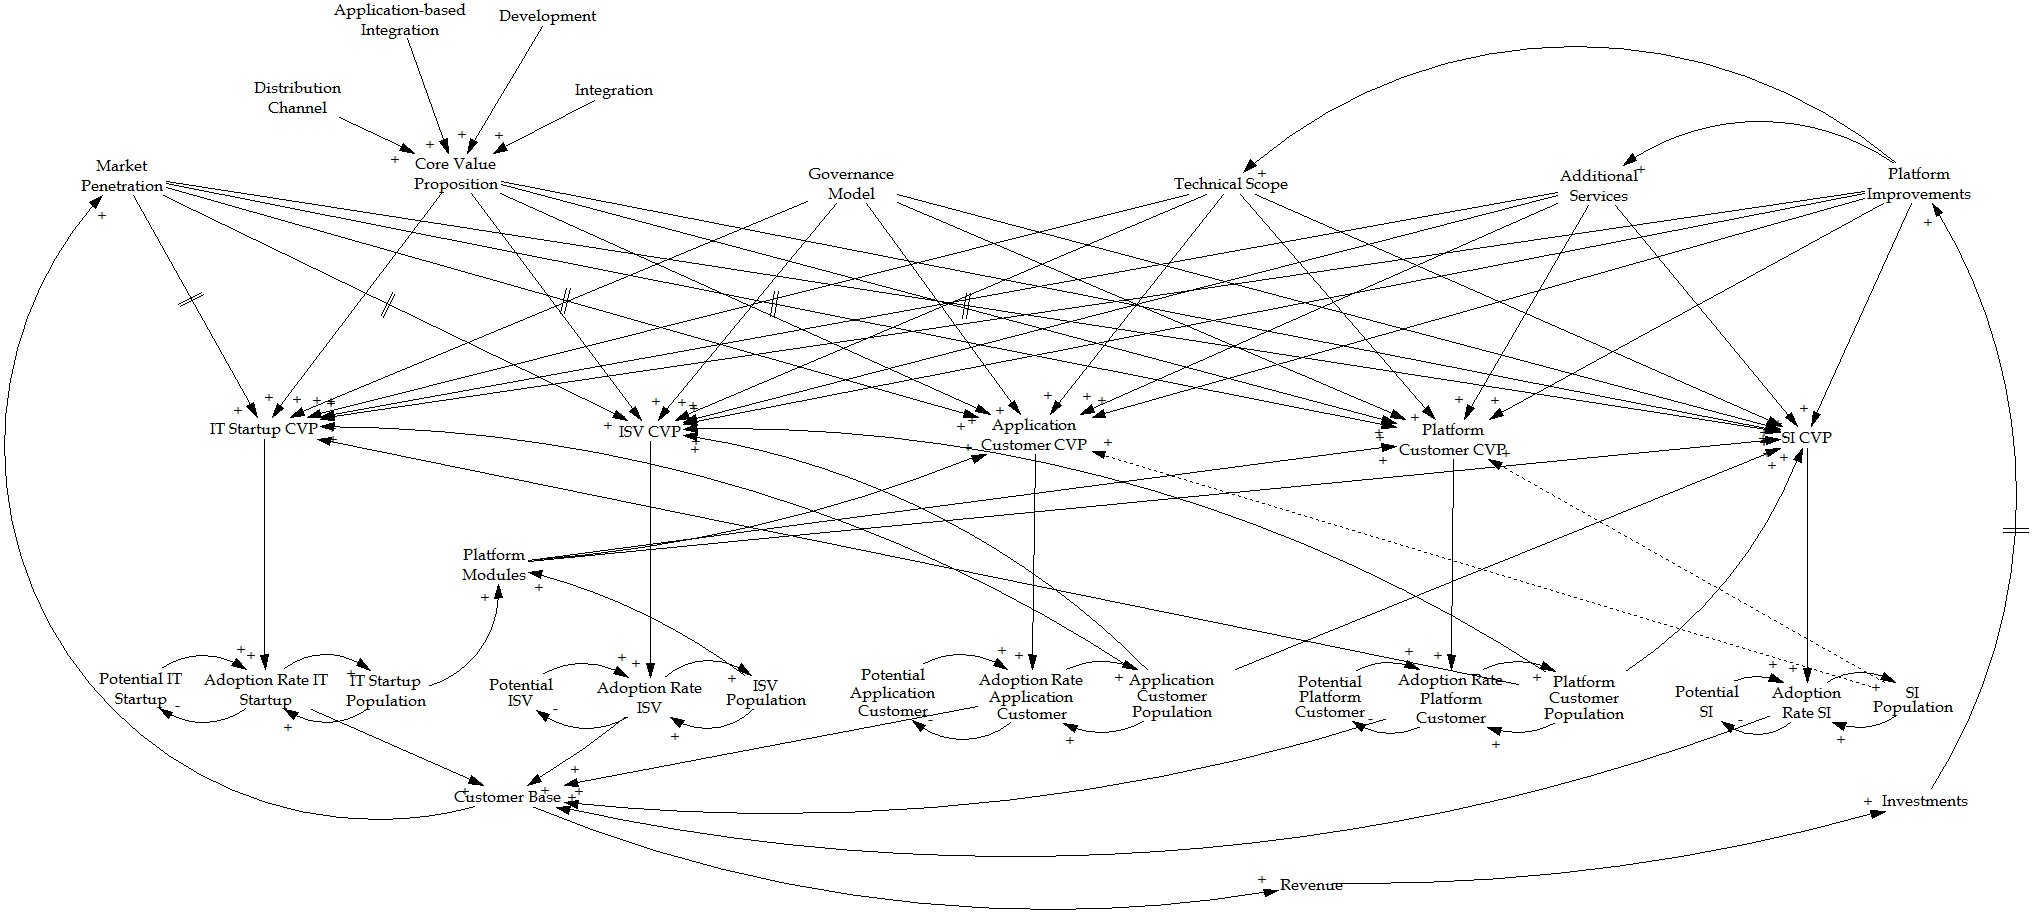
\includegraphics[width=0.96\textheight,angle=270]{gfx/cld_bigPicture}
		\caption{Causal Loop Diagram -- The Big Picture}
		\label{fig:cld_bp}
	\end{figure}
}



